\chapter{Theory}

This chapter describes the underlying concepts which are used throughout the thesis. 

\section{OpenStreetMap Data Model}\label{openstreetmap_data_model}

The data model of \osm{} consists of objects of type node, way and relation. Nodes define points in space, ways define linear features and relations define how objects relate to each other\cite{1_osm_wiki_2016}.

\begin{figure}[H]
    \centering
    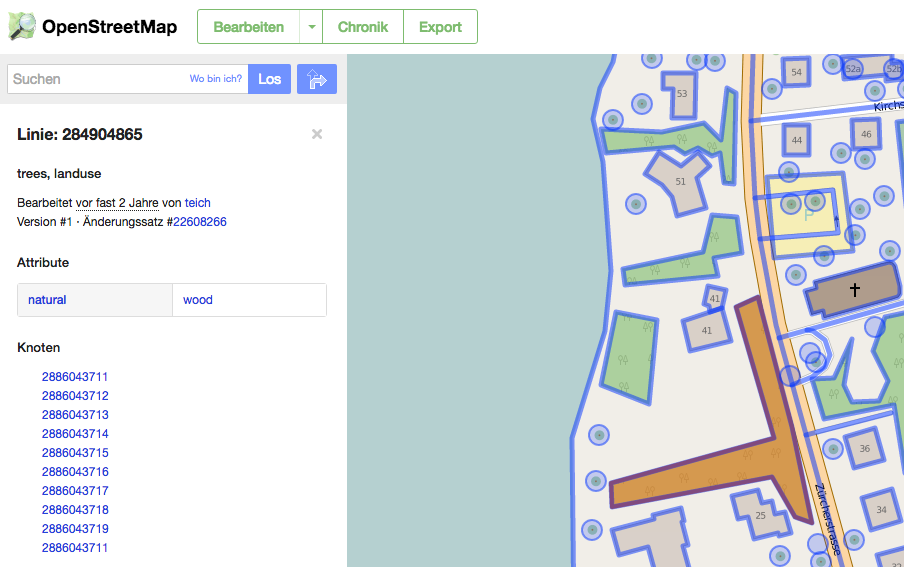
\includegraphics[width=1\textwidth]{images/osm_data_model}
    \caption{Example of object tagged natural=wood}
    \label{landuse_on_osm_editor}
\end{figure}

Every object can have one or more tags associated with it. Tags define the meaning of a certain object. A tag consists of a key/value pair for example the tag \textbf{natural=wood} is used to define areas which are covered in trees. \osm{} tags are not strictly defined and users can add their own tags but there are many conventions which should be followed.\\

The semi-structured \osm{} data model is transformed a structured database schema as explained in \autoref{sub_import_mapping}. Nodes, ways and relations are converted into real geometries.
A way for example is turned into a polygon because it is a closed way where the first and last node are shared\cite{13_osm_wiki_closed_way}.

\section{Vector Tiles}\label{part1_vector_tiles}

Instead of delivering a image of the map to a client like a browser or mobile phone, only the vector representation of the data is sent to the client which is using less data and allows more interactive, dynamic  and resolution independent cartography. This is only possible since clients have more powerful hardware and are able to render maps themselves.

\begin{figure}[H]
\centering
\includegraphics[width=1.0\textwidth]{images/vector_raster_example}
\caption{Vector and client representation of a map section}
\end{figure}
    

\noindent\begin{minipage}[t]{0.48\linewidth}
    \vspace{0pt}
    Google introduced the XYZ tiling scheme \cite{v_1_wiki.openstreetmap.org_2015} back in 2005 because it is not scalable to deliver an image of the map tailored to the viewport of the client.
    The idea is to divide the map image into a grid as shown in \autoref{tiled_raster_map} where clients request idempotent raster images by using tile indizes instead of coordinates. This allows caching on the browser and server side and results in a smoother map experience.
    The same approach can be applied to vector data. Instead of delivering the vector data for the entire viewport the vector data is sliced into tiles.\\\\
    Vector tiles contain all the geometry and metadata needed for a specific tile. This makes them more flexible than serving raster tiles, because a different style can be applied on the fly. For example based on the language preference of the browser language-specific city labels can be shown.
\end{minipage}
\hfill
\begin{minipage}[t]{0.48\linewidth}
    \vspace{-10pt}
    \begin{figure}[H]
        \centering
        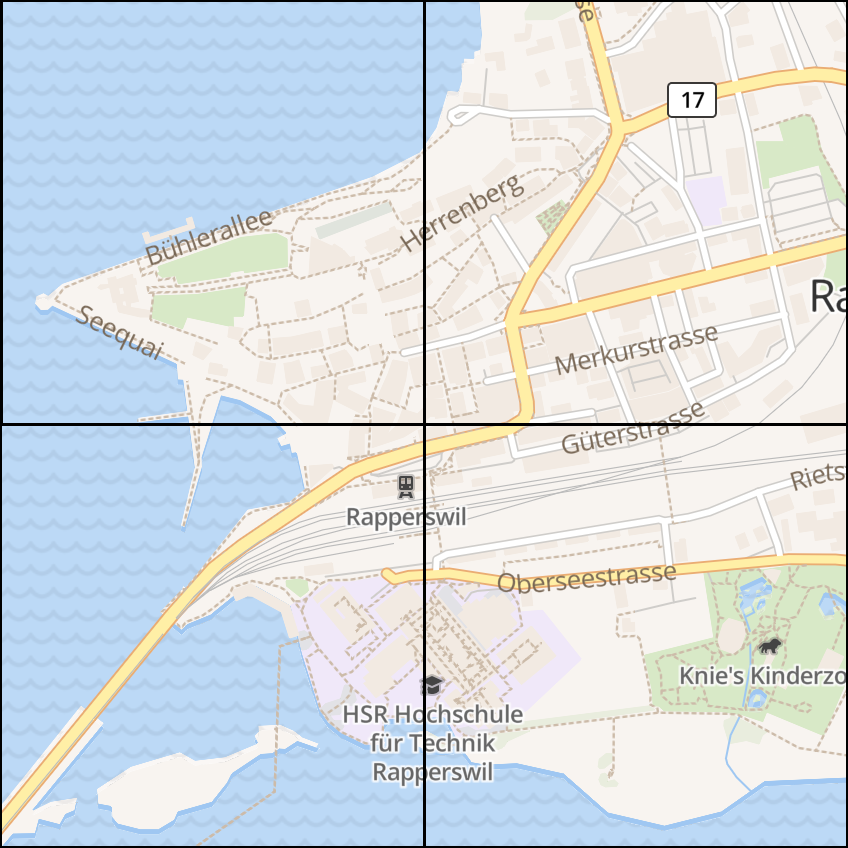
\includegraphics[width=\textwidth]{images/tiled_raster}
        \caption{Tiled raster map}
        \label{tiled_raster_map}
    \end{figure}
\end{minipage}


\section{Mapbox Vector Tile Specification}\label{part1_vector_tile_specification}
    
The Mapbox Vector Tile Specification defines how to encode tiled vector data using Protocol Buffers\cite{protobuf_2016}. More details about the encoding and internal structure of vector tiles can be found in the specification\cite{104_mapbox.com_2016}.\\

%\subsection*{Vector Tile Structure}\label{part1_vector_tile_structure}

The data inside of vector tiles is structured into layers and features. A vector tile can have multiple layers such as roads, landuse or water (elaborated in \autoref{database-schema}). Each layer consists of one or multiple features and must have a unique name. A feature contains a geometry field (either of type point, linestring or polygon) and metadata (tags) such as label translations. The metadata key-value pairs are stored in the layer as arrays of keys and values. The tags on the feature only reference the key and value by their index. This helps to keep the file size small since only the unique values and keys need to be stored and can be referenced by multiple features.
Keys can only be strings while values can have different types such as string, double or integer. 


\begin{figure}[H]
    \centering
    \includegraphics[width=\textwidth]{images/vector_tile_structure}
    \caption{Vector Tile Structure}
    \label{vector_tile_structure}
\end{figure}

The \textbf{extent} field defines the width and height of the tile coordinates (the vector tile resolution) which is relevant for encoding the geometry of a feature as shown in \autoref{vector_tile_grid}. For \osmvt{} the resolution of 4096 coordinate units has been chosen.

%\subsection*{Geometry Encoding}\label{part1_geometry_encoding}

\noindent\begin{minipage}[t]{0.48\linewidth}
    \vspace{0pt}
    The geographic coordinates of the geometries are converted into relative coordinates inside the vector tile.
    Vector tiles are encoded as commands for a virtual pen (the rendering client). Drawing the polygon from \autoref{vector_tile_grid} results in the commands from Listing \autoref{encoded_commands}.
    
    \begin{enumerate}
        \item Move to the starting point $(3,1)$ relative to the top left corner
        \item Draw line from current pen position to $(3,3)$. Since the target position is encoded relative to the current position the encoded geometries take up less space.
        \item Draw line from current position $(6,4)$ to $(-4,2)$ 
        \item Close path of current position $(2,6)$ with last used starting point $(3,1)$
    \end{enumerate}
\end{minipage}
\hfill
\begin{minipage}[t]{0.48\linewidth}
    \vspace{-20pt}
    \begin{figure}[H]
        \centering
        \includegraphics[width=\textwidth]{images/vector_tile_grid}
        \caption{Vector tile grid with encoded geometry}
        \label{vector_tile_grid}
    \end{figure}
    \vspace{-10pt}
    \begin{listing}[H]
\begin{plpgsqlcode}
LineTo(3,1)
LineTo(3,3)
LineTo(-4,2)
ClosePath()
\end{plpgsqlcode}
        \caption{Geometry inside vector tile encoded as drawing commands}
        \label{encoded_commands}
    \end{listing}
\end{minipage}





\section{XYZ Coordinate Schema}\label{part1_xyz_coordinates}

\noindent\begin{minipage}[t]{0.48\linewidth}
    \vspace{0pt}
    For tiling the vector tiles the XYZ numbering schema has been used.
    The tiles are organized in a 3-dimensional coordinate system (\texttt{x/y/z}) where \texttt{x} and \texttt{y} represent the axes and \texttt{z} the zoom level. As users zoom into a map each tile is replaced by four children within the tile.\\\\
    The map in mercator projection is divided into the x and y axis. The x axis reaches from 0 to $2^z$ (from left to right edge of map) and the y axis from 0 to $2^z$ (from top to bottom edge of map).
\end{minipage}
\hfill
\begin{minipage}[t]{0.48\linewidth}
    \vspace{-10pt}
    \begin{figure}[H]
    \centering
    \includegraphics[width=\textwidth]{images/xyz_scheme}
    \caption{XYZ coordinate schema}
    \end{figure}
\end{minipage}

